\documentclass[a4paper,12pt]{article}
\usepackage[margin=2cm]{geometry}
\usepackage[utf8]{inputenc}
\usepackage{natbib}
\usepackage{amsfonts}
\usepackage{amsmath}
\usepackage{graphicx}
\usepackage{parskip}
\usepackage{color}
\usepackage{algpseudocode}
\usepackage{algorithm}
\usepackage{minted}
\usepackage{url}
\usepackage{hyperref}
\usepackage{amssymb}
\usepackage{pgf}

% Turn off section numbering
\setcounter{secnumdepth}{0}

% Disable hideous fluorescent links
\hypersetup{hidelinks = true}

% Custom macros
\newcommand{\MultiGraph}{\texttt{MultiGraph }}
\newcommand{\Graph}{\texttt{Graph }}
\newcommand{\OStar}{O^*}

\title{COMP6741 Assignment 2}
\author{Magnus Hagmar (z5088131)
    \and
    Michael Sproul (z3484357)}
\date{October, 2015}

\begin{document}
\maketitle
\pagenumbering{arabic}

\section{Q1 - Feedback Vertex Set Algorithm 1}
Our implementation of the algorithm described in Parameterized Algorithms~\cite{parameterized} can be found in the file \textbf{fvs.py} and is called \textbf{fvs\_via\_ic}.

\section{Q2 - Feedback Vertex Set Algorithm 2}
The second algorithm we chose is the one described in section 6.2 of Exact Exponential Algorithms~\cite{exactexp}. It is also found in \textbf{fvs.py} and is called \textbf{fvs\_via\_mif}.

\section{Q3 - Implementation}

Our implementation is written in Python 3 and makes use of the NetworkX v1.10 \cite{networkx} graph library for basic graph operations. In particular, we use the \MultiGraph type extensively, which models an undirected graph in which multiple edges are allowed between any two vertices. The reason for using a \MultiGraph rather than a regular undirected \Graph is that both algorithms require the ability to create multiple edges between vertices. Under the hood, \MultiGraph is implemented using several nested dictionaries, which are themselves implemented as hash-tables. This allows edge and vertex look-ups and many other operations to be performed with good amortised time complexity. For example, a graph $G$ with edges $\{(1, 2), (1, 2)\}$ is expressed as a \MultiGraph as follows:

\begin{minted}{python}
>>> g = MultiGraph(data=[(1, 2), (1, 2)])
>>> g.edges()
[(1, 2), (1, 2)]
>>> g.adj
{1: {2: {0: {}, 1: {}}}, 2: {1: {0: {}, 1: {}}}}
\end{minted}

Note how the adjacency dictionary (\texttt{g.adj}) stores each edge twice - once as a mapping from 1 to 2 and once as a mapping from 2 to 1. This requires more space but importantly allows any vertex's neighbours to be enumerated quickly (if each edge were stored only once the entire graph would need to be traversed). The inner dictionaries mapping 0 and 1 to \texttt{\{\}} represent the fact that the edge $(1, 2)$ appears twice. NetworkX allows any hashable type to be used as a label, and allows metadata to be stored on edges and vertices, but for our purposes we only make use of integer labels, and ignore metadata entirely.

When running a profiler on our algorithms, we discovered that our greatest loss of performance was caused by copying of the graph and other function parameters. We have attempted to minimize the amount of copying by passing a reference to the original graph where no mutation is required. Where branching into sub-cases which will modify the graph, a copy is created to avoid mutation.

Upon further consideration, we have come up with another change which should increase performance significantly. If we could avoid copying elements altogether then we would gain a massive boost in speed. This could be achieved by using some kind of version control for the graph. This way, we could modify it for use in a recursive call, and then easily restore it to its earlier state upon completion of the recursive call. The simplest way this could be implemented is using a list to store the changes being made so that they can be reverted later.


\subsection{FVS via Iterative Compression}

The implementation of the iterative compression algorithm consists of functions for solving \textsc{Disjoint-FVS} and \textsc{FVS-Compression}, as well as \textsc{FVS} itself. The function for \textsc{FVS} (\texttt{fvs\_via\_ic}) is a straight-forward translation of the high-level algorithm -- iteratively expanding and compressing an initially trivial solution. When solving the compression problem on subgraphs, NetworkX's \texttt{subgraph} method is used, which copies the relevant nodes and edges. In this case its use cannot impact the running time too much, as only $O(n)$ iterations of this loop are performed. The implementation function for \texttt{FVS-Compression} (\texttt{ic\_compression}) includes graph copying with a greater impact on performance, as its loop runs over $O(2^k)$ subsets. Optimising the \texttt{graph\_minus} function that computes $G - W$ for use in each of these $O(2^k)$ sub-problems yielded an approximate 2$\times$ speed-up on some instances! Our current approach builds a graph up whilst ignoring vertices from $W$, which is significantly faster than the naive approach of copying the entire graph and removing vertices from $W$ (see \texttt{graph\_minus\_slow}).

In \texttt{ic\_compression}'s loop, $O(2^k)$ calls to the function for \textsc{Disjoint-FVS} (\texttt{fvs\_disjoint}) do most of the work. We say that calling \texttt{fvs\_disjoint(g, w, k)} \textit{passes ownership} of \texttt{g} to the function -- meaning that \texttt{fvs\_disjoint} has a unique reference to \texttt{g} and is allowed to mutate it freely. The reductions were initially written in a functional-style, so that a new copy of the graph was returned whenever a reduction was successfully applied. However, given that the original graph is never considered after applying the reductions and \texttt{fvs\_disjoint} has ownership of it, it is safe to use mutation. Although one might expect the use of mutation to drastically reduce the amount of copying, we found that it did not yield significant performance improvements, most likely due to the reductions only accounting for a small part of the overall run-time. After applying the reductions, the algorithm select a vertex $x \in H$ of degree 1 or less using a simple polynomial time loop. The algorithm then branches on whether $x$ is included in the solution being found, or not. In the case where $x$ is included, the graph is effectively copied to create $G - \{x\}$ for the recursive call. In the case where $x$ is not included, the algorithm recurses on $G$, which can be passed without copying as \texttt{g} is owned by \texttt{fvs\_disjoint} and is not needed again. Hence it is necessary to create a copy of the graph only for 1 of the 2 recursive calls.

In spite of our efforts to reduce copying, profiling reveals that copying data still accounts for the most significant portion of the iterative compression algorithm's run-time. We suspect that reducing copying through a transactional system as sketched above could provide greatly improved performance. Combined with a language that compiles to machine-code, we suspect an implementation with a running time approximately 100 times faster would be within reach.

\begin{verbatim}
   ncalls       tottime  percall  cumtime  percall  filename:lineno(function)
2583028/77780   3.344    0.000    7.695    0.000    copy.py:137(deepcopy)
735214/77780    1.429    0.000    5.556    0.000    copy.py:242(_deepcopy_dict)
   708934       1.176    0.000    1.254    0.000    multigraph.py:255(add_edge)
    10279       0.829    0.000    3.267    0.000    fvs.py:16(graph_minus)
   101282       0.746    0.000    1.609    0.000    multigraph.py:1003(subgraph)
\end{verbatim}

Iterative compression profiling results (top 5, k = 10).

\subsection{FVS via Maximum Induced Forest}

The implementation our second algorithm calculates a feedback vertex set by solving the \textsc{maximum induced forest} problem, as described in Exact Exponential Algorithms~\cite{exactexp}. It consists primarily of three functions: two preprocessing procedures as well as the main procedure. All procedures are translations of the described algorithm, with one addition. The algorithm presented in the book strives to calculate a \textit{minimum} feedback vertex set rather than answer the question of whether one of size at most $k$ exists. Our implementation passes along an integer $k$ denoting how many more vertices must be included in the forest before the fvs will be small enough. As soon as a sufficiently large forest (and thereby small fvs) has been calculated, the algorithm will return to avoid unnecessary calculations. This change improves performance in many cases, but will not improve cases where the graph consists of more than one connected component. In these cases it is impossible to know how many vertices are to be included in the forest from each component, so the algorithm will revert to finding an induced forest of maximum size.

Similarly to our algorithm using iterative compression, we make sure to only copy the graph (and other elements) when recursive calls are going to mutate them. Despite this, it is clear from running a profiler that copying is taking the most time, as shown below. In addition to copying, the other three most time-consuming functions are all part of NetworkX. Even greater performance improvements could most likely be gained by using a different graph implementation.

In particular, a lot if time is spent on the compression step, as it is run many times when calculating the generalized degree of vertices and it is one of the cases where the graph is copied. This is where we could gain the most by improving the graph handling to avoid copying.

\begin{verbatim}
   ncalls     tottime percall cumtime percall filename:lineno(function)
1974290/16999 3.231   0.000   7.453   0.000   copy.py:137(deepcopy)
  1505878     2.558   0.000   3.449   0.000   connected.py:205(_plain_bfs)
710682/16999  1.843   0.000   6.644   0.000   copy.py:242(_deepcopy_dict)
   119927     1.279   0.000   2.851   0.000   multigraph.py:1003(subgraph)
   444874     1.204   0.000   4.891   0.000   connected.py:26(connected_components)
\end{verbatim}

Maximum induced forest profiling results (top 5, k = 15)

\section{Q4 - Instance Generation}

The algorithm that we use to generate instances to test our algorithms is called \textbf{generate\_custom} and can be found in the file \textbf{generate.py}. It accepts two parameters which can be used to adjust the graph size and the minimum size of the feedback vertex set. The first parameter is simply the desired size of the FVS, $k$. Generating graphs in this manner gives us the advantage of always knowing whether our instance will be a yes or no instance every time we run the algorithms. This way, we can easily test cases where $k$ is much smaller than, almost equal to, equal to and much greater than the actual size of the FVS and compare their performance. The second parameter, $q$, is used to tweak how large the graph is in comparison to its minimum FVS. A large value for this second value with a small $k$ will generate graphs with a high number of vertices while still having a small FVS, and vice versa.

The way in which the actual graph is generated is by creating a series of disjoint connected components, followed by linking these together with edges between random vertices. Each component is, however, only attached to the main graph by a single edge, so that no unpredicted cycles are introduced. As such, our generator will only generate connected graphs. We reasoned that this would not be an issue, as both of our chosen algorithms will compute a FVS for a disconnected graph $G$ by simply running on each connected component of $G$. As long as a correct result can be provided for each individual component, then the answer for the graph as a whole will be correct as well.

The connected components which are created can be one of three types. The first is either a simple path or a single vertex. These components are used to increase the size of the graph without increasing the size of the minimum FVS. The second type of component is a cycle, which of course increases the size of the FVS by one. Both the length of the paths and cycles depend on the second parameter to \textbf{generate\_custom}, which is how the size of the graph is controlled. Finally, the last type of components which we use are complete graphs -- a complete graph on $n$ vertices has a minimum FVS size of $n - 2$ for $n \geq 3$. Intuitively, it should be these complete graph components that contribute most to the difficulty of an instance.

There are some limitations to this method of generating graphs, however. There are some structures of graphs which we are unable to generate. One such graph is cycles with internal edges, such as $\{(0,1),(1,2),(2,3),(3,0),(0,2)\}$. The reason that we still consider our solution viable is the massive advantage of knowing the size of the minimum FVS in advance when testing. Our method of generation has a very wide coverage and should, together with the known value of $k$, provide sufficient test cases to properly analyse the algorithms.

\section{Q5 - Performance}

We tested our algorithms against several sets of generated instances, mostly with $k$ set to the size of the minimum feedback-vertex-set. To determine whether \textsc{Yes} or \textsc{No} instances were more difficult we also ran a smaller set of tests with $k$ set to 1 less than the size of the minimum feedback-vertex-set.

\subsection{Testing Environment}

The testing environment's specifications were as follows:

\begin{itemize}
\item \textbf{CPU:} Intel(R) Xeon(R) CPU E5-2630L v2 @ 2.40GHz (one core).
\item \textbf{RAM:} 512MB
\item \textbf{OS:} Linux x86\_64, kernel version 3.8.4
\item Python v3.4.3
\item NetworkX v1.10
\end{itemize}

Although this is quite a small amount of memory for a computationally intensive task, we found that our generated instances required no more than around 30MB of RAM. It is also worth noting that the tests were run within a virtualisation environment, on a DigitalOcean server.

To measure algorithm execution time, we opted to write our own timing function as Python's recommended benchmarking library -- \texttt{timeit} -- is more focused on timing static code than code that takes different inputs. The \texttt{time\_instance} function in \texttt{benchmark.py} instead uses the simple \texttt{time.process\_time} Python library function to measure the time elapsed while solving a single instance with a given algorithm. \texttt{time.process\_time} measures the total time that the process has spent actually executing, which is preferable to wall-time as it eliminates time when the process isn't scheduled and running. From the documentation for \texttt{time.process\_time}: \textit{return the value (in fractional seconds) of the sum of the system and user CPU time of the current process. It does not include time elapsed during sleep}.

To time a collection of instances, we used a process-pool as this allows us to set a timeout of 10 minutes for any single task. We set the pool size to 1 to ensure serial execution (recall that the test machine only has a single core). This code can be found in \texttt{time\_all} in \texttt{benchmark.py}.

We made extensive use of Python's serialisation capabilities to store problem instances and results. All of the files in the \texttt{data} and \texttt{results} directories can be deserialised using the \texttt{from\_disk} function located in \texttt{generate.py}. The \texttt{gather\_data.py} script was used to orchestrate the solving of pre-generated instances loaded from \texttt{data}.

\subsection{Instances with known $k$}

Given limited time for testing, we chose to run the algorithms with $k$ set to the minimum FVS size, as this intuitively gives a sense of the algorithm working to its potential -- trying to find the smallest possible feedback-vertex-set. In preliminary testing we found that instances with $k = 16$ were about as large as either algorithm could handle in less than 10 minutes. We optimistically generated three sets with small, medium and large numbers of vertices, but in practice found that only the small graphs were solvable by both algorithms. Their specifications are given below:

\begin{tabular}{|l|l|l|l|l|l|}
\hline
\textbf{Name} & \textbf{$k$ min.} & \textbf{$k$ max.} & $q$ & \textbf{Avg. $n$} & \textbf{Number} \\ \hline
small & 1 & 16 & 16 & $\approx$ 80 & 80 \\ \hline
medium & 1 & 16 & 50 & $\approx$ 200 & 80 \\ \hline
large & 1 & 16 & 200 & $\approx$ 400 & 80 \\ \hline
\end{tabular}

The iterative compression (IC) algorithm is FPT, with a running time of $\OStar(5^k)$, whilst the MIF algorithm is not and has a running time of $\OStar(1.899^n)$. As such when plotting running time against $k$ one would expect IC running time to ascend exponentially and MIF running time to grow more slowly. Our results are as follows:

\begin{figure}[h!]
\centering
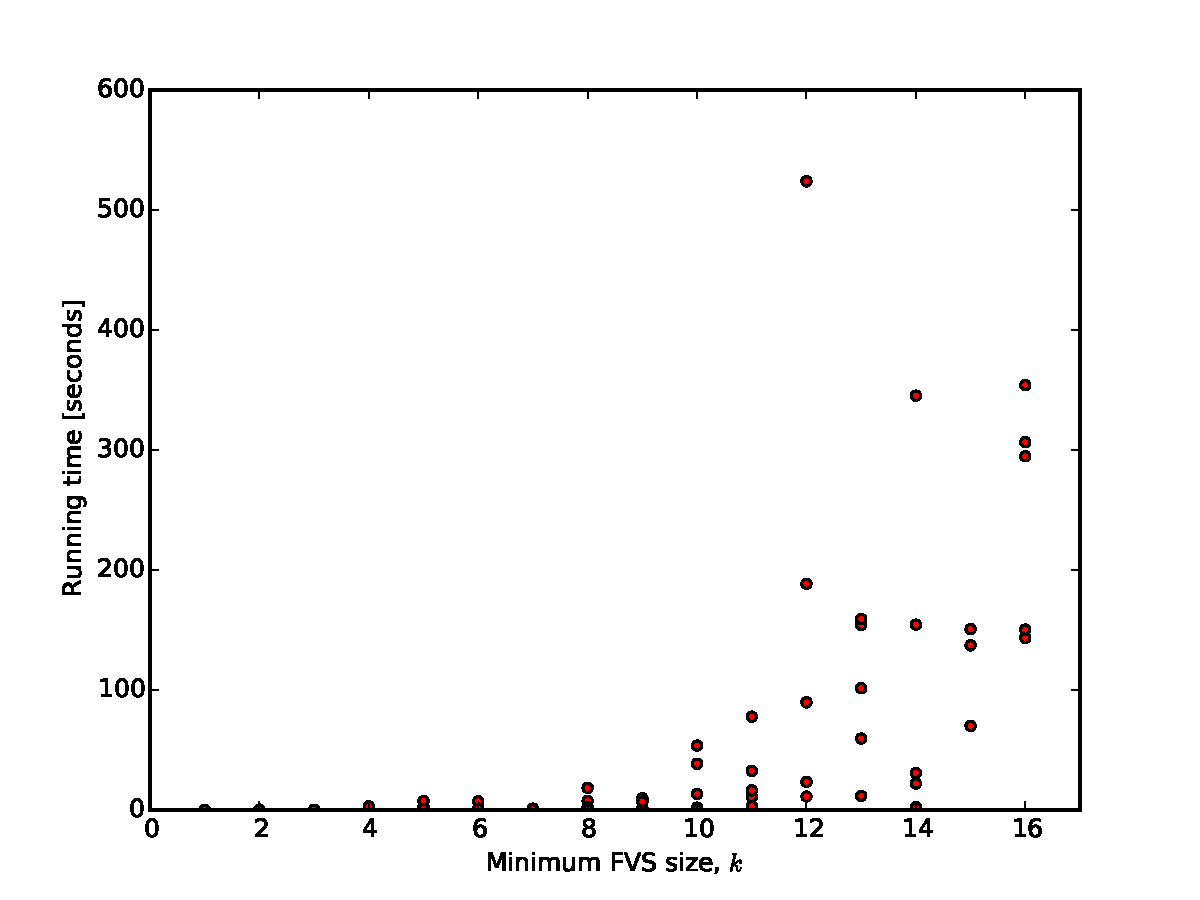
\includegraphics[width=15cm]{ic_small_k.pdf}
\caption{IC Running time vs $k$.}
\label{fig:ic_small_k}
\end{figure}

\begin{figure}[h!]
\centering
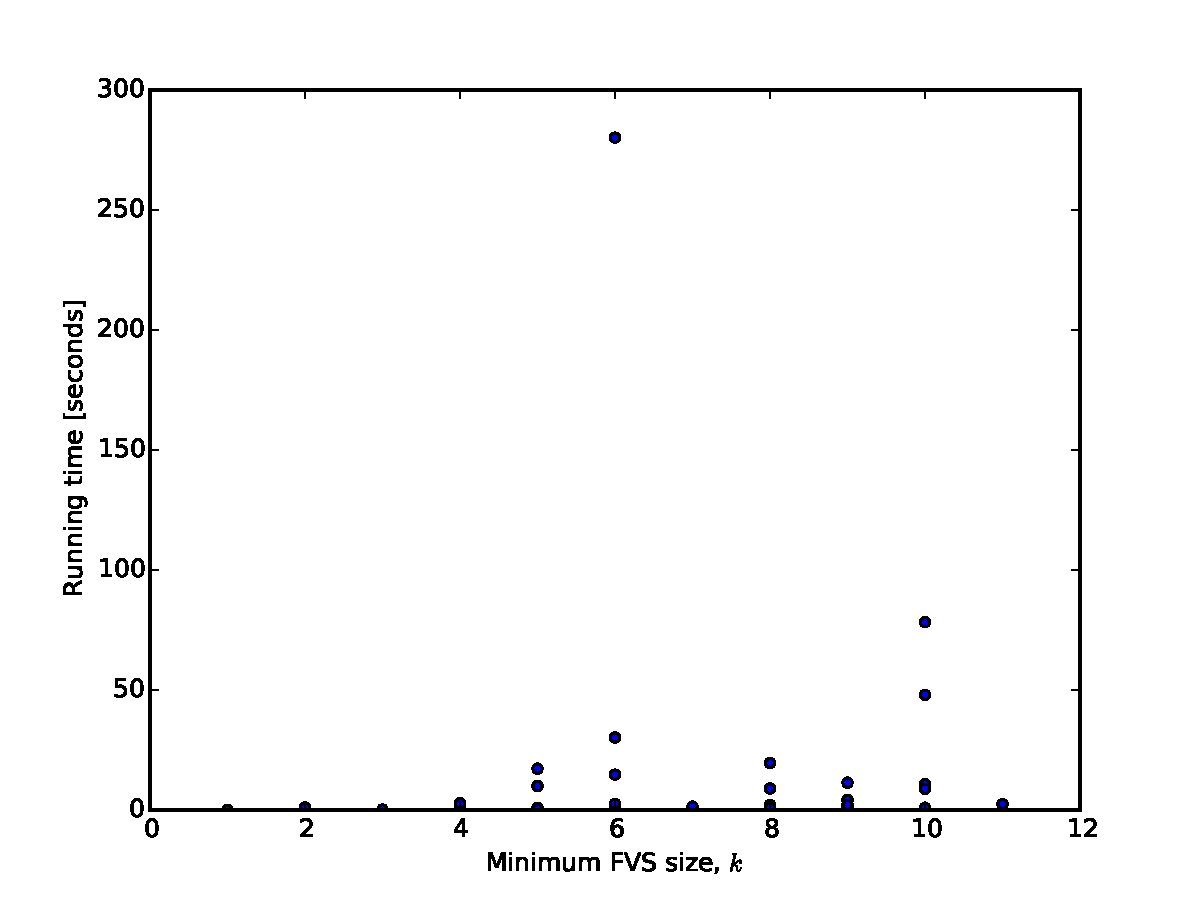
\includegraphics[width=15cm]{mif_small_k.pdf}
\caption{MIF Running time vs $k$.}
\label{fig:mif_small_k}
\end{figure}

\pagebreak

For the iterative compression algorithm, only 2 of the 80 instances timed out. Both instances that timed out had $k = 15$ and considerable numbers of vertices (140 and 260). Like the outlier at $k = 12$, there doesn't seem to be anything distinguishing these instances from the others, except that they have large values of $k$ and moderately large numbers of vertices. Some of the solved $k = 12$ and $k = 15$ vertices have larger numbers of vertices than the catastrophic instances (the largest $n$ being 320). Further proof that $n$ is not the source of the increase can be found in the graphs of running time against $n$ (Figures \ref{fig:ic_small_n}, \ref{fig:mif_small_n}).

In the case of the MIF algorithm, almost all instances with $k$ larger than 10 timed out. Notably, the tests were run before a significant last-minute optimisation (the use of mutation in \texttt{compress}), and we didn't have time to re-compute the entire data set. However, from testing a few of the timed out instances we think the results would be more or less the same.

The general trend in the data for the IC algorithm approximately matches our expectation of exponential growth. If anything, the growth is \textit{less} rapid than expected, which is likely due to computational overhead not associated with $k$ (e.g. large amounts of copying due to large numbers of vertices). Unfortunately, without a more sophisticated instance generation method capable of creating instances with fixed $n$ and $k$, we were unable to keep $n$ constant whilst varying $k$. This is particularly significant when considering the data for the MIF algorithm, as the graphs with larger $k$ tend to also have larger $n$, leading to the unexpected time-outs for larger $k$ values (recall that we expect MIF's running time to grow only in proportion to some polynomial in $k$).

Further, consider the plots of running time against the number of vertices for both algorithms. Contrary to the previous plots, theory dictates that IC's running time should grow slowly in $n$ (as it is FPT), whilst MIF's should grow exponentially. In the results for IC (Figure \ref{fig:ic_small_n}) observe that there is very little correlation except that larger values of $n$ weakly imply larger running times. We attribute this to overhead from graph copying operations, discussed previously.

In the results for MIF's running time plotted against $n$ (Figure \ref{fig:mif_small_n}) the expected exponential growth is unfortunately absent. We attribute this to the larger instances timing out. For the 29/80 instances that MIF timed out on, the mean number of vertices is approximately 157. Were these instances allowed to be solved in times greater than 10 minutes, the plot would exhibit the expected exponential structure. To concretely capture the relationship, the algorithm could be allowed to run for longer, or else slightly smaller instances could be selected (with around 100 to 120 vertices).

To summarise, we observed the expected theoretical behaviour for IC's running time plotted against $k$ and attributed IC's unexpected growth in running time with $n$ to a straight-forward property of the implementation (lots of graph copying). Futher, we found the plot of MIF's running time against $k$ to be inconclusive, and argued that the plot for MIF's running time against $n$ matches the theory when the timed-out instances are considered.

Considering which instances seemed particularly hard to solve, we tested several properties of the instances that timed-out or took a long time. The number of edges seems not to impact the running time of either algorithm too significantly, except that it is typically accompanied by larger $n$ and hence larger $k$ (due to how our instances were generated). The maximum degree of any vertex also proved to be an insignificant factor.

\begin{figure}
\centering
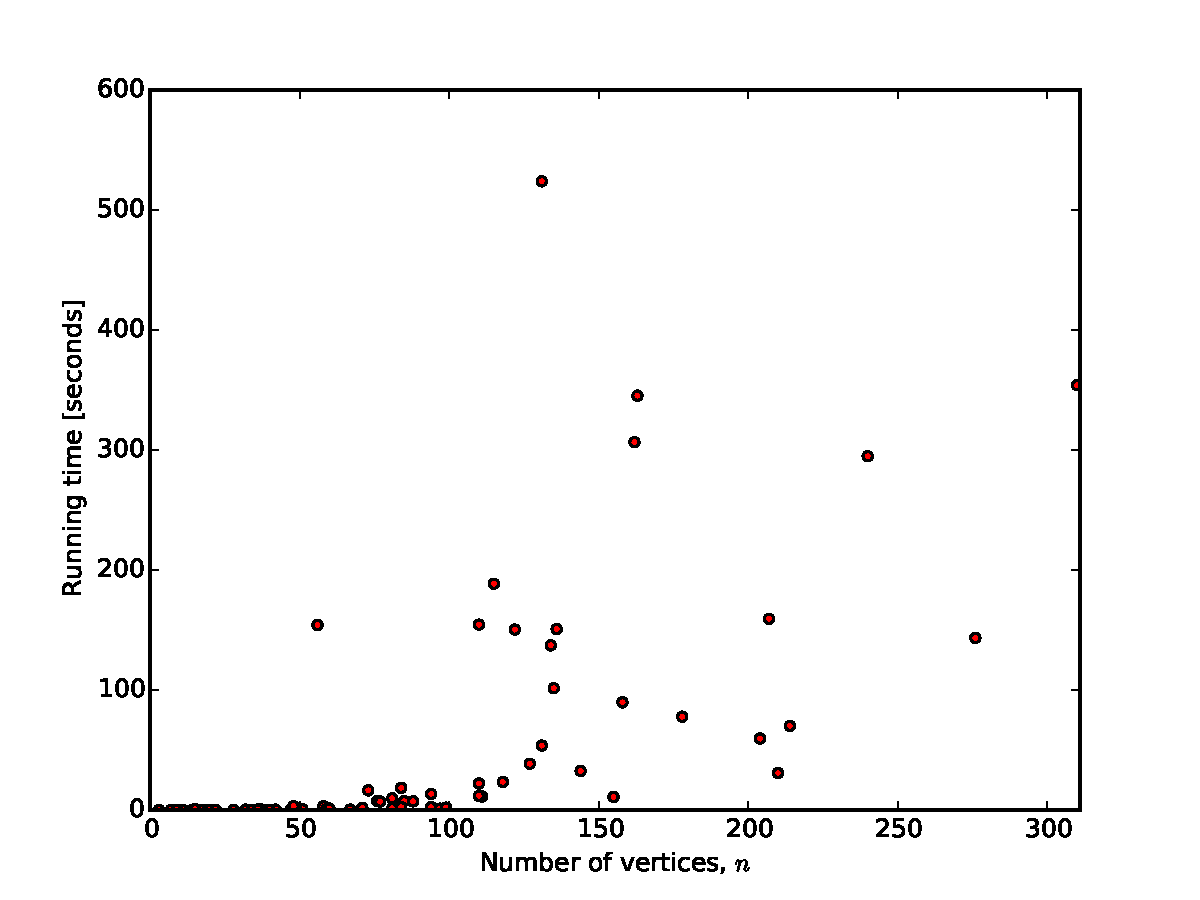
\includegraphics[width=15cm]{ic_small_n.pdf}
\caption{IC running time vs $n$}
\label{fig:ic_small_n}
\end{figure}

\begin{figure}
\centering
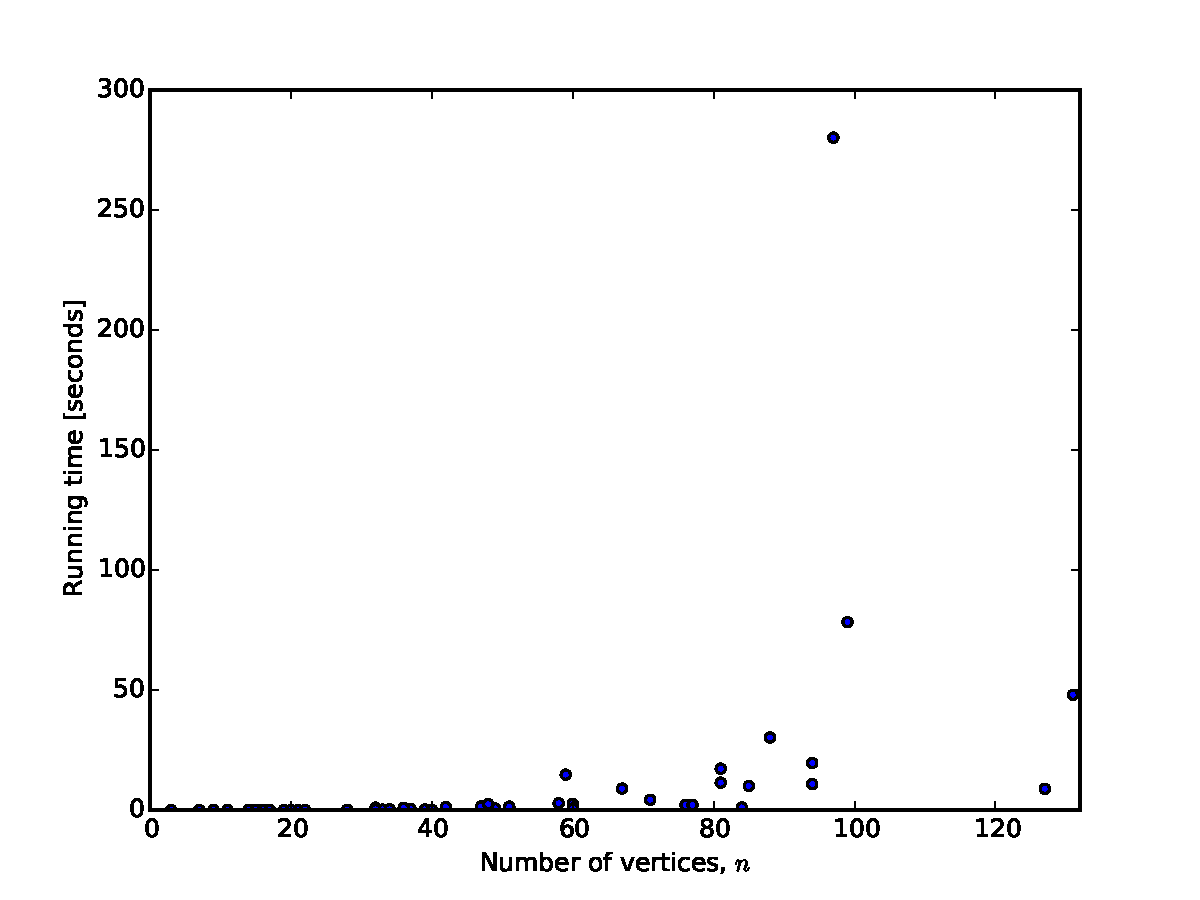
\includegraphics[width=15cm]{mif_small_n.pdf}
\caption{MIF running time vs $n$}
\label{fig:mif_small_n}
\end{figure}

\pagebreak

\subsection{Yes and No instances}

To test our algorithms and compare performance for YES and NO instances, we simply ran a series of test cases with $k$ set to both the size of the minimum FVS, as well as the minimum size minus one. 

For the MIF algorithm, it seems that for small instances a NO instance will run slightly faster than a YES instance. As instance size grows, YES instances get relatively faster. This is due to the algorithm returning the found MIF (and FVS) as soon as one is discovered rather than continuing to find a smaller one. This behaviour was expected and not very surprising. In figure \ref{fig:mif_yes_no}, the relative running time of YES and NO instances of the same graph are shown. As one can see, when the instance size grows the data points start to tend towards the negative, indicative of YES instances taking comparatively less time.

\begin{figure}[h]
\centering
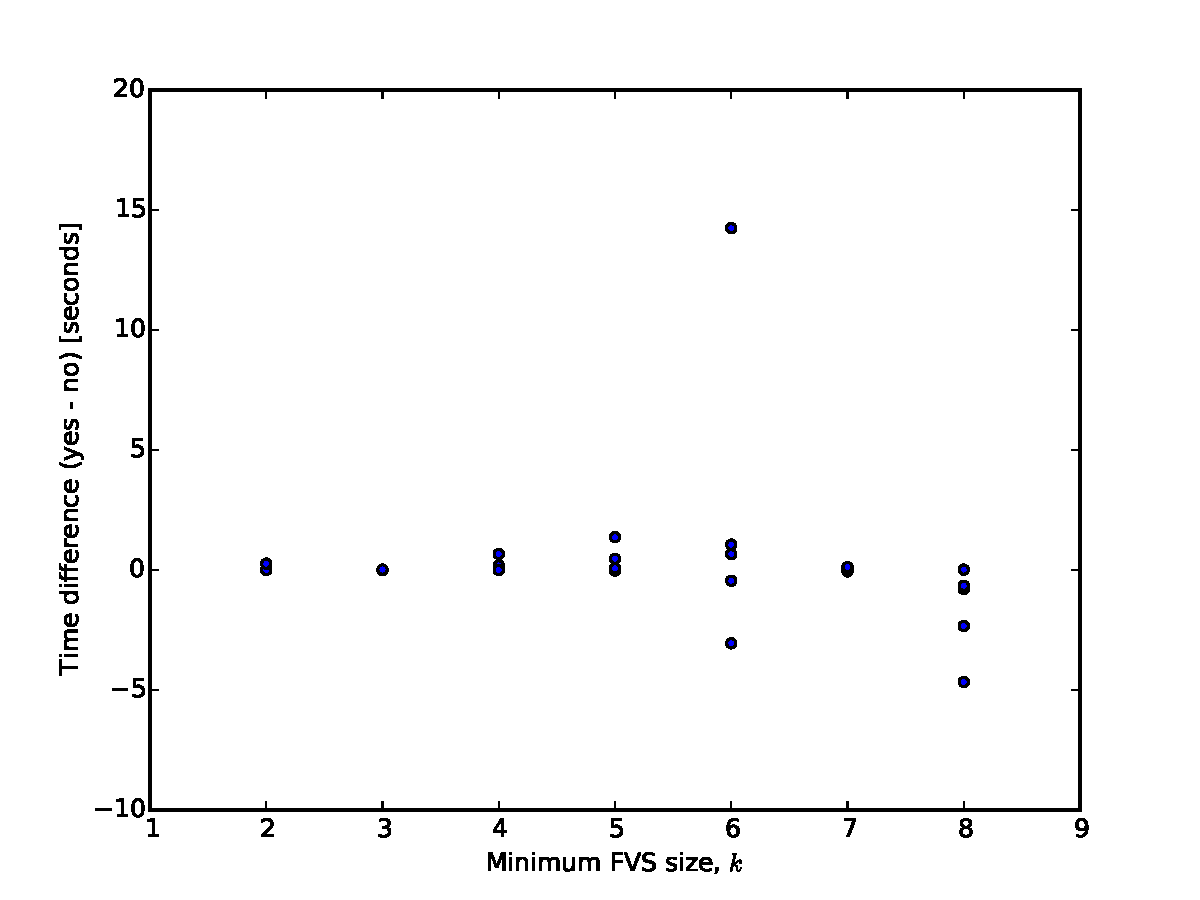
\includegraphics[width=15cm]{mif_yes_no.pdf}
\caption{Difference in MIF running times for YES and NO instances.}
\label{fig:mif_yes_no}
\end{figure}

For the IC algorithm, it seems that YES instances are easier to solve, as indicated by a sharp trend towards the negative in Figure \ref{fig:ic_yes_no}. This is in contrast to the MIF algorithm, which generally solves NO instances more easily. We take this as mild evidence that NO instances are more difficult to solve for the IC algorithm, at least when $k$ is 1 less than the minimum FVS size. One explanation for this effect could be that the algorithm has to work harder at each stage to find solutions to the disjoint FVS problem (as it is looking for smaller solutions), yet still runs for almost as many iterations as the algorithm that succeeds with $k = k^*$.

Note that the graphs used for the YES/NO tests are a subset of the \textit{small} dataset, with $k$ between 2 and 8.

\begin{figure}[h]
\centering
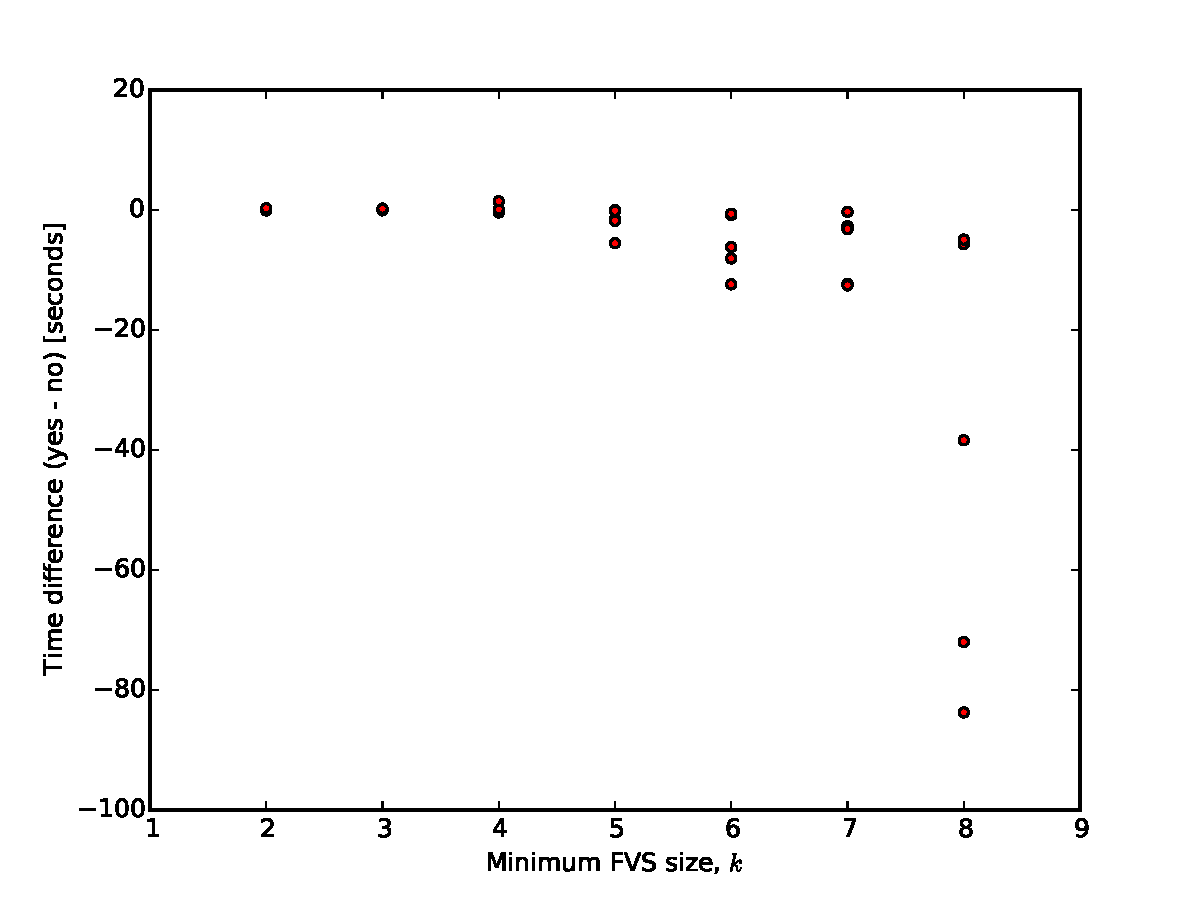
\includegraphics[width=15cm]{ic_yes_no.pdf}
\caption{Difference in IC running times for YES and NO instances.}
\label{fig:ic_yes_no}
\end{figure}

% References
\pagebreak
\bibliographystyle{unsrt}
\bibliography{references}

\end{document}

